% One particle-mesh step as a loop of six operations. \lit picks the lit one: 0 lights all six,
% 1..6 one at a time (paint, FFT, IFFT, read forces, interpolate to the particles, kick and drift).
% Compile: see ../build.sh (seven renders to PNG, composed with the particles by pm_run.py).
\documentclass[tikz,border=6pt]{standalone}
\usepackage{tikz}
\usepackage{amsmath}
\usepackage{bm}
\usepackage[T1]{fontenc}
\usetikzlibrary{arrows.meta,positioning,calc}
\providecommand{\lit}{0}
\definecolor{ink}{HTML}{2E2E2E}
\definecolor{greytx}{HTML}{9A9A9A}
\definecolor{kw}{HTML}{C2560A}
\definecolor{litfill}{HTML}{FBE7D6}
\definecolor{panel}{HTML}{F4F6FA}
\newcommand{\stylefor}[1]{\ifnum\lit=0 lit\else\ifnum\lit=#1 lit\else dim\fi\fi}
\begin{document}
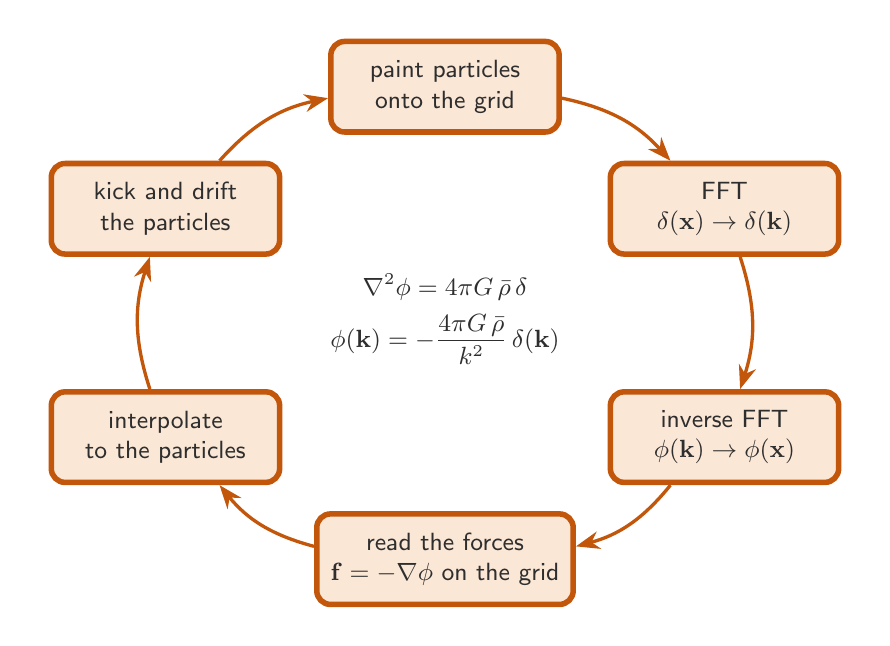
\begin{tikzpicture}[font=\sffamily,
  base/.style={rounded corners=5pt,inner sep=5pt,align=center,font=\sffamily\small,
               minimum width=2.9cm,minimum height=1.15cm},
  lit/.style={base,draw=kw,line width=2pt,fill=litfill,text=ink},
  dim/.style={base,draw=greytx,line width=0.9pt,fill=panel,text=greytx},
  pmarrow/.style={-{Stealth[length=3mm]},kw,line width=1.2pt}]
  \useasboundingbox (-5.3,-3.75) rectangle (5.3,3.75);
  \node[\stylefor{1}] (paint) at (0,3.0) {paint particles\\onto the grid};
  \node[\stylefor{2}] (fft) at (3.55,1.45) {FFT\\$\delta(\mathbf{x}) \to \delta(\mathbf{k})$};
  \node[\stylefor{3}] (ifft) at (3.55,-1.45) {inverse FFT\\$\phi(\mathbf{k}) \to \phi(\mathbf{x})$};
  \node[\stylefor{4}] (force) at (0,-3.0) {read the forces\\$\mathbf{f} = -\nabla\phi$ on the grid};
  \node[\stylefor{5}] (interp) at (-3.55,-1.45) {interpolate\\to the particles};
  \node[\stylefor{6}] (adv) at (-3.55,1.45) {kick and drift\\the particles};
  \draw[pmarrow] (paint) to[bend left=18] (fft);
  \draw[pmarrow] (fft) to[bend left=18] (ifft);
  \draw[pmarrow] (ifft) to[bend left=18] (force);
  \draw[pmarrow] (force) to[bend left=18] (interp);
  \draw[pmarrow] (interp) to[bend left=18] (adv);
  \draw[pmarrow] (adv) to[bend left=18] (paint);
  \node[ink,font=\sffamily\small,align=center] at (0,0.05)
       {$\nabla^2\phi = 4\pi G\,\bar\rho\,\delta$\\[4pt]
        $\phi(\mathbf{k}) = -\dfrac{4\pi G\,\bar\rho}{k^2}\,\delta(\mathbf{k})$};
\end{tikzpicture}
\end{document}
